%%%%%%%%%%%%%%%%%%%%%%%%%%%%%%%%%%%%%%%%%%%%%%%%%%%%%%%%%%%%%%%%%%%%%%%%%%%%%%%

\chapter{APÊNDICE F - Programa FORTRAN 90 Filtro Recusrivo 1D/2D}
\label{apendiceVI}

O programa abaixo foi escrito em linguagem FORTRAN 90 para resolver as equações que representam o Filtro Recursivo 1D e 2D Homogêneo. Segundo Purser et al., 2003a, a melhor caracterização da curva Gaussiana simulada pelo filtro recursivo, dá-se pelo filtro de quarta ordem, mas devido à complexidade das equações, apenas a primeira e a segunda ordem foram implementadas, para efeito de estudo e compreensão do Filtro Recursivo. O programa utiliza a biblioteca LAPACK para a decomposição das matrizes $A$ e $B$. A Figura 25, apresenta o resultado do Filtro Recursivo a partir de um sinal inicial aleatório, com diferentes valores de $\alpha$.

\begin{figure}[!h]
\centering
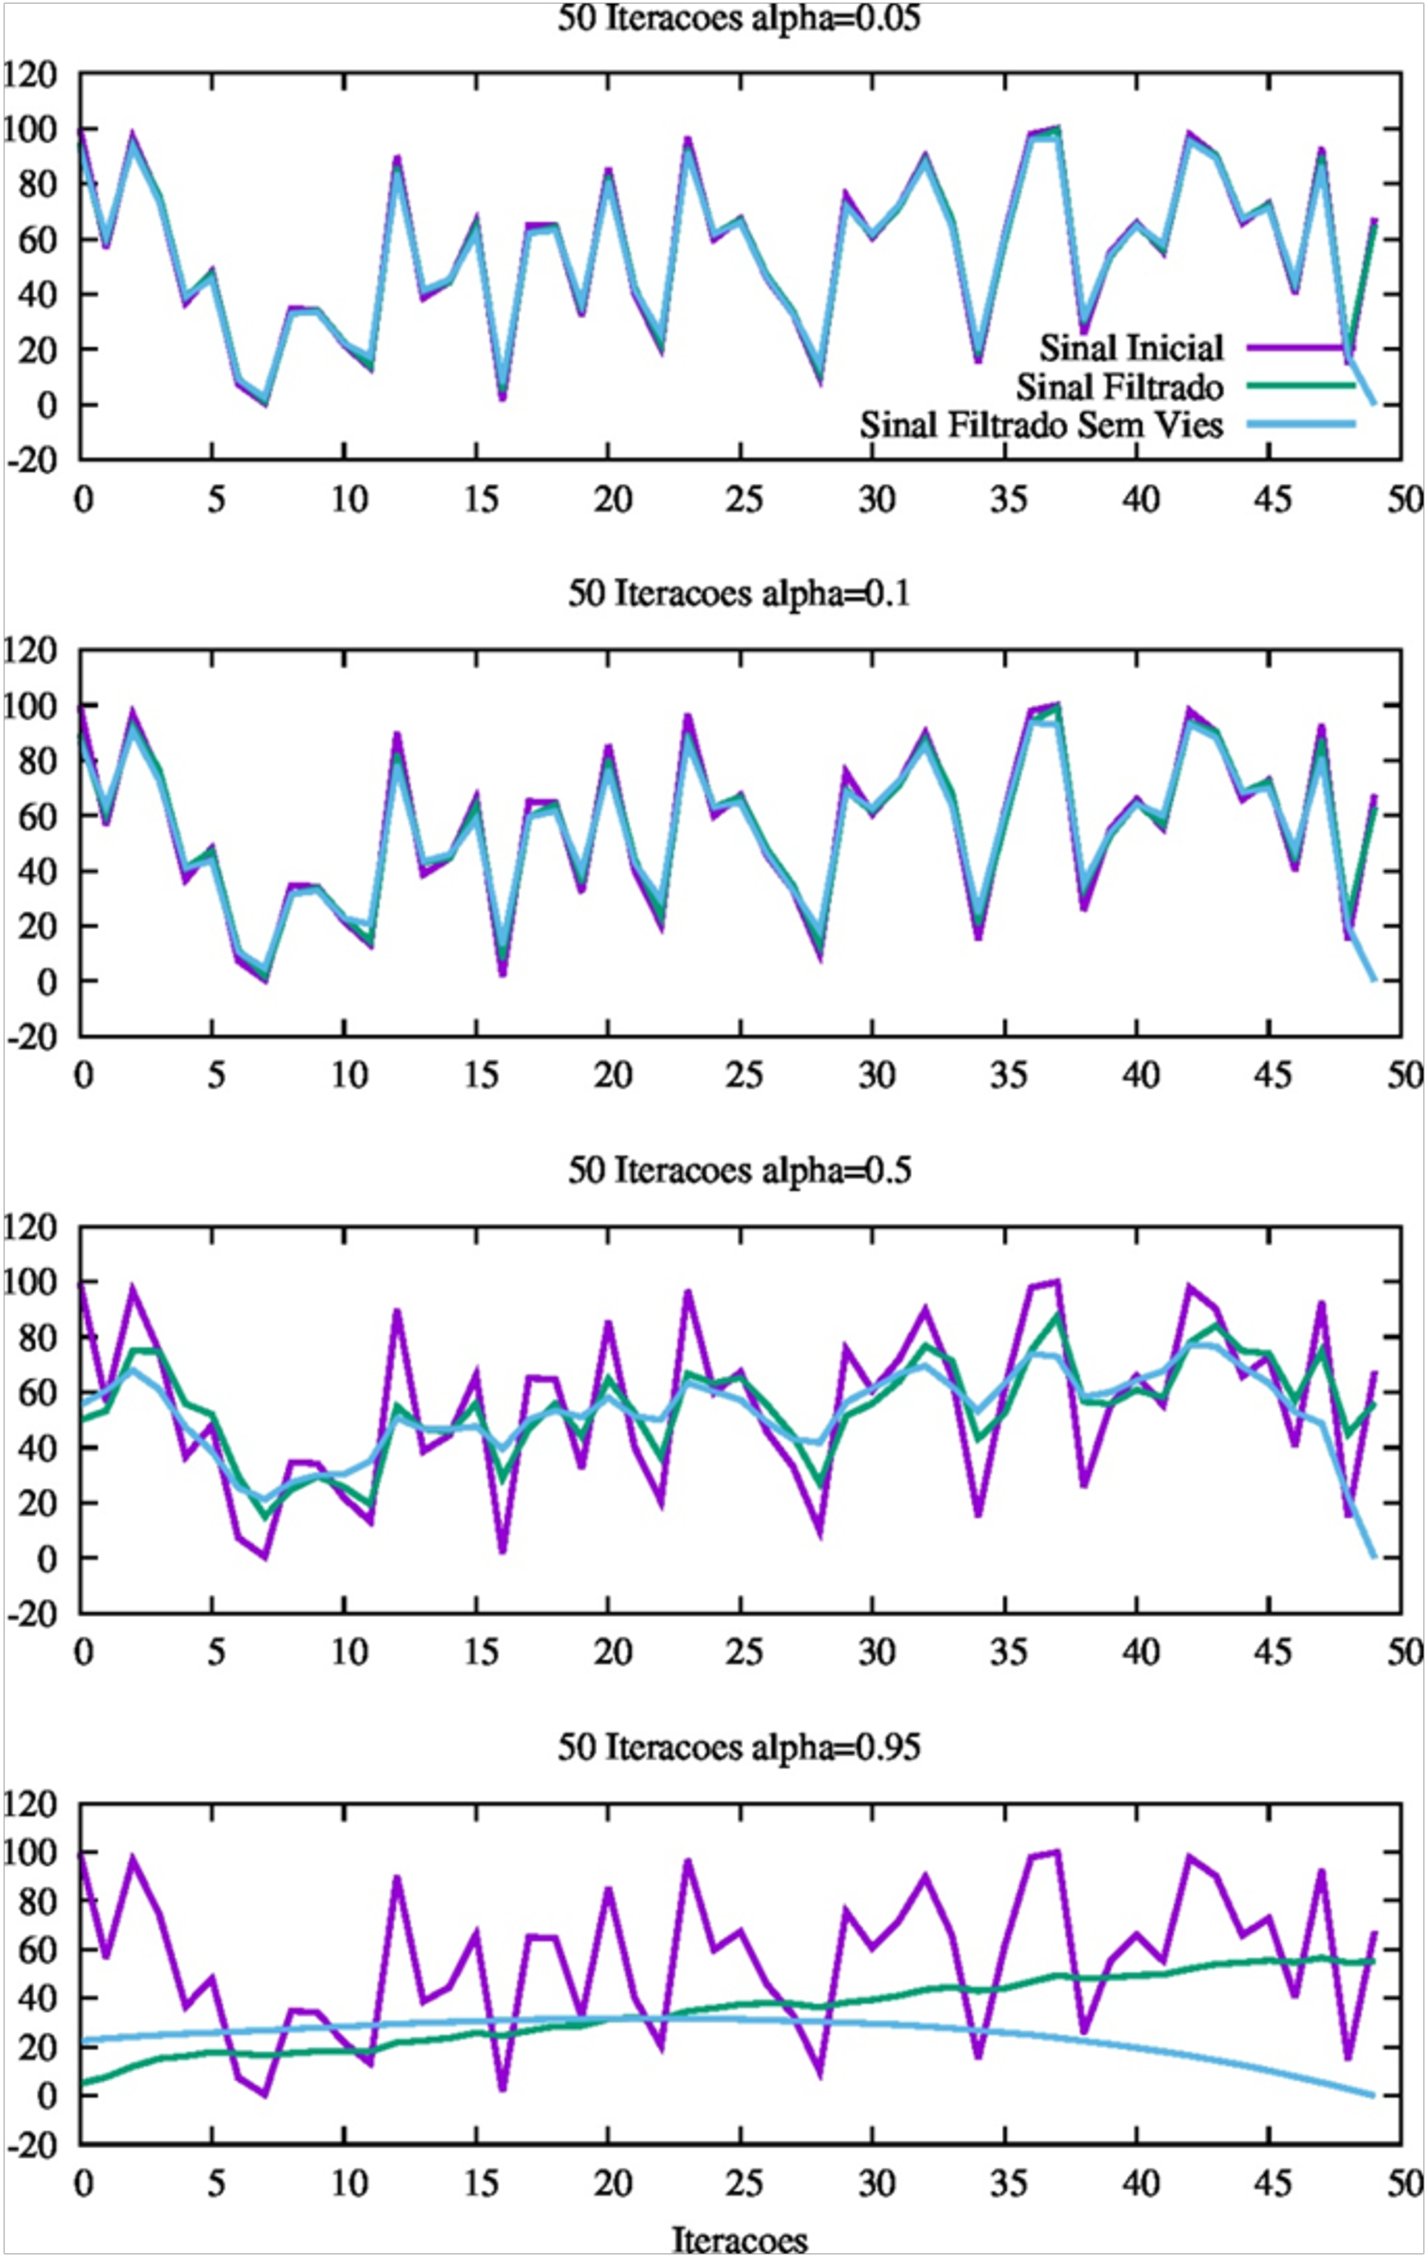
\includegraphics[clip,trim=0 0 0 0,scale=0.4]{./figs/ap3/filtro_rec_1d.pdf}
\caption{Simulação Filtro Recursivo a partir de um sinal inicial aleatório, com diferentes valores para $\alpha$, em 50 iterações.}
\end{figure}

% \begin{lstlisting}[label=some-code,caption=Código fonte do Filtro Recursivo 1D]
% ! Unidimensional Homogeneous Recursive Filter
% ! Purser et al., 2003a
% !
% ! Instructions (complile/execute/plot):
% ! $ gfortran rec_filter.f90 -L/opt/lapack-3.5.0_gcc-4.8.8 -llapack -lblas
% ! $ ./a.out 
% !
% ! Results are written to p.txt, q.txt and s.txt files
% ! Visualize the results using the accompanion script (depends on gnuplot):
% ! $ gnuplot plot_filter_results.gpl
% !
% ! Carlos Frederico Bastarz
% ! March, 2015

% program rec_filter

%   implicit none

%   integer            :: i, j         ! i and j are counters
%   integer            :: k            ! k is a counter
%   integer            :: info         ! info is an output code (used by DGESV and DPSTF2)
%   integer            :: rank         ! rank returns the rank of matrix D (used by DPSTF2)

%   integer, parameter :: dims=1       ! dims is the filter's dimension (at this time it is only unidimensional) \
%                                      ! so, any other value here will have no effect
%   integer, parameter :: m=11         ! m is the number of points over a line grid (use odd values >= 3)
%   integer, parameter :: fo=1         ! fo is the filter order, must be 1, 2 or 4
%   integer, parameter :: input=2      ! input is the input type: 1 = unit; 2 = Gaussian
%   integer, parameter :: npass=1      ! npass is the number os passes: 1 is 1 forward and 1 backward pass
%   integer, parameter :: gaussopt=2   ! gaussopt: 1 - uses m to compute mean and standard deviation \
%                                      !           2 - use arbitrary values to shape the Gaussian Function \
%                                      !           (see subroutine gauss_input for more options) \
%                                      ! Obs: this option will only take effect when input=2

%   real(8), parameter :: dx=4.        ! dx is the grid spacing
%   real(8), parameter :: aa=8.        ! aa is a convenient measure of the instrinsic \
%                                      ! distance scale of the smooth filter
%                                      ! aa is the standard deviation for the initial impulse - have to be fixed, \
%                                      ! making it dependent on Gaussin input

%   real(8)    :: sigma                ! sigma is the ratio between aa and dx
%   real(8)    :: w1, w2               ! w1 and w2 are the coefficients of a z quadratic eq. (in terms of kappa)
%   complex(8) :: k1, k2               ! k1 and k2 are a polynomial's roots (in terms of sigma)
%   complex(8) :: z1, z2, z            ! z1 and z2 are the roots of the z quadratic eq.
%                                      ! z is the smallest root between z1 and z2

%   real(8) :: modz1, modz2            ! modz1 and modz2 are the moduli of z1 and z2

%   real(8), dimension(m)   :: s, p, q ! q is a initial unit impulse input \
%                                      ! (it changes later on) to the forward system \
%                                      ! it is also the output of the backward system \
%                                      ! s is the input impulse to the forward system

%   real(8), dimension(m)   :: Zf      ! Zf is the forward shift operator
%   real(8), dimension(m)   :: Zb      ! Zb is the backward shift operator
%   real(8), dimension(m,m) :: A       ! A is the forward factor of D2 (actually is a triangular A)
%   real(8), dimension(m,m) :: B       ! B is the backward factor of D2 (actually is a triangular B)
%   real(8), dimension(m,m) :: A1      ! Full A
%   real(8), dimension(m,m) :: B1      ! Full B

%   real(8), dimension(m) :: A2, B2

%   real(8), dimension(m,m) :: D       ! D is the covariance contribution (D=A*B) \
%                                      ! also, the diagonals of D has the filter's coeeficients (alphas and betas)
   
%   real(8), dimension(m)   :: pivot   ! pivot is an array that records the pivoting of the linear systems (used by DGESV)
%   real(8), dimension(m,m) :: W       ! W is a work matrix used in the Cholesky factorization (used by DPSTF2)



%   character(100) :: fmt              ! fmt is a write format character

%   fmt="(30F16.8)"                    ! output format: 30 numbers with 16 digits and 8 decimal points

% ! Begin:

%   call check_parameters(m,input,fo,gaussopt)

%   call print_options(dims,fo,m,dx,aa,input,npass,gaussopt)

%   ! sigma:
%   sigma=aa/dx

%   print *
%   print *, "sigma:"
%   write(*,(fmt)) sigma

%   ! Filter Order (1, 2, or 4 - as of May'2015, 4th order is still not available):
%   if(fo.eq.1)then

%     ! k1:
%     k1=cmplx(-2./sigma**2,0)

%     print *
%     print *, "k1:"
%     write(*,(fmt)) k1

%     ! w1:
%     w1=1+(1/sigma**2)

%     print *
%     print *, "w1:"
%     write(*,(fmt)) w1

%     ! z1:
%     z1=cmplx(w1,sqrt(w1**2-1))

%     ! z2:
%     ! If z=a+bi, we can calculate the inverse of z as:
%     ! z^-1=(a-bi)/(a**2+b**2)
%     ! or simply by:
%     ! z^-1=1/z
% !    z2=1/z1
%     z2=conjg(z1)/(realpart(z1)**2+imagpart(z1)**2)

%     print *
%     print *, "z1, z2:"
%     write(*,(fmt)) z1, z2

%     ! Pick up the smallest zp (z1 or z2):
%     ! - Calculate the moduli of z1 and z2
%     modz1=sqrt((realpart(z1)**2)+(imagpart(z1)**2))
%     modz2=sqrt((realpart(z2)**2)+(imagpart(z2)**2))  
  
%     print *
%     print *, "modz1, modz2:"
%     write(*,(fmt)) modz1, modz2

%     if(modz1.gt.modz2)then
%       z=z2
%     else
%       z=z1
%     end if

%     print *
%     print *, "z:"
%     write(*,(fmt)) z

%     ! Stability criteria: 
%     ! z<1 or -1<modz<1
    
%     ! - Check for modz1:
% !    if(modz1.ge.1.or.modz1.le.-1)then
% !      stop "modz1 is greather or equal 1 or is less or equal -1."
% !    end if

%     ! - Check for modz2:
% !    if(modz2.ge.1.or.modz2.le.-1)then
% !      stop "modz2 is greather or equal 1 or is less or equal -1."
% !    end if

%     ! We initializate A2 and B2 with zeroes:
%     A2=0.
%     B2=0.
  
%     ! Shift Operators (Zf and Zb):
%     do k=1, m
  
%       Zf(k)=k ! Zf is the forward part
  
% !      A2(k)=(1-z*Zf(k))/(1-z)
%       A2(k)=(1-z)/(1-z*Zf(k))
  
%       Zb(k)=(m+1)-k ! Zb is the backward part
  
% !      B2(k)=(1-z*Zb(k))/(1-z)
%       B2(k)=(1-z)/(1-z*Zb(k))
  
%     end do

%     ! Fill up the lower triangular of A1 with A2, so that the diagonals of A1
%     ! are a repetition of the indices of A2, ie., we want something like this 
%     ! (eg, for A2=[1 2 3 4 5]^T):
%     !      |1   0    0    0    0|
%     !      |2   1    0    0    0|
%     ! A1 = |3   2    1    0    0|
%     !      |4   3    2    1    0|
%     !      |5   4    3    2    1|
%     A1=0. ! Initialize A1 with zeroes
%     do i=1, m
%       do j=1, m
%         k=i-j+1
%         if(i.ge.j)then
%           A1(i,j)=A2(k)
%         end if
%       end do
%     end do
  
%     ! And now, fill up the upper triangular of B1 with B2, so that the diagonals of B1
%     ! are a repetition of the indices of B2, ie., we want something like this 
%     ! (eg, for B2=[-1 -2 -3 -4 -5]^T):
%     !      |0  -1   -2   -3   -4|
%     !      |0   0   -1   -2   -3|
%     ! B1 = |0   0    0   -1   -2|
%     !      |0   0    0    0   -1|
%     !      |0   0    0    0    0|
%     B1=0. ! Initialize B1 with zeroes
%     k=1
%     do i=1, m
%       do j=1, m
%         if(j-i.eq.k)then
%           B1(i,j)=B2(k)
%           k=k+1
%         else if(j-i.eq.1)then
%           B1(i,j)=B2(j-i)
%         else if(j-i.gt.1)then
%           B1(i,j)=B2(j-i)
%         end if
%       end do
%     end do

%     ! Construct matrix D using the A1 and B1, so that:
%     !     |1  -1   -2   -3   -4|
%     !     |2   1   -1   -2   -3|
%     ! D = |3   2    1   -1   -2|
%     !     |4   3    2    1   -1|
%     !     |5   4    3    2    1|
%     D=A1+B1

%     ! Should I do D=matmul(A1,B1) and then use Cholesky factorization to get A and B?
% !    D=matmul(A1,B1)

% !!  else if(fo.eq.2)then ! This is specific for the second order filter (not complete yet)
% !!
% !!    ! k1:
% !!    k1=cmplx((-6*sigma**2)/(sigma**2+3*sigma**4),(12/sigma**2+3*sigma**4)*sqrt((3*sigma**4+2*sigma**2)/12)) 
% !!
% !!    ! k2:
% !!    k2=cmplx((-6*sigma**2)/(sigma**2+3*sigma**4),(-12/sigma**2+3*sigma**4)*sqrt((3*sigma**4+2*sigma**2)/12)) 
% !!  
% !!    print *
% !!    print *, "k1, k2:"
% !!    write(*,(fmt)) k1, k2
% !!  
% !!    ! w1:
% !!    w1=cmplx(1+(3*sigma**2/sigma**2+3*sigma**4),(-6/sigma**2+3*sigma**4)*sqrt((3*sigma**3+2*sigma**2)/12)) 
% !! 
% !!    ! w2:
% !!    w1=cmplx(1+(3*sigma**2/sigma**2+3*sigma**4),(6/sigma**2+3*sigma**4)*sqrt((3*sigma**3+2*sigma**2)/12)) 
% !!  
% !!    print *
% !!    print *, "w1, w2:"
% !!    write(*,(fmt)) w1, w2
% !!  
% !!    ! z1:
% !!    z1=cmplx(w1,sqrt(w1**2-1)) 
% !!
% !!    ! z2:
% !!!    z2=1/z1
% !!    z2=conjg(z1)/(realpart(z1)**2+imagpart(z1)**2)
% !!     
% !! 
% !!    print *
% !!    print *, "z1, z2:"
% !!    write(*,(fmt)) z1, z2
% !!  
% !!    ! Pick up the smallest zp (z1 or z2):
% !!    ! - Calculate the moduli of z1 and z2
% !!    modz1=sqrt((realpart(z1)**2)+(imagpart(z1)**2))
% !!    modz2=sqrt((realpart(z2)**2)+(imagpart(z2)**2))
% !!    
% !!    print *
% !!    print *, "modz1, modz2:"
% !!    write(*,(fmt)) modz1, modz2
% !!
% !!    if(modz1.gt.modz2)then
% !!      z=z2
% !!    else
% !!      z=z1
% !!    end if
% !!
% !!    ! A1, B1:
% !!    do i=1, m ! forward
% !!      do j=m, 1, -1 ! backward 
% !!  
% !!        ! Zf:
% !!        Zf(i)=i ! Z**-1
% !!  
% !!        ! Zb:
% !!        Zb(i)=j ! Z
% !!  
% !!        ! A1: first pass
% !!        A1(i,j)=((1-z1*Zf(i))*(1-z2*Zf(i)))/((1-z1)*(1-z2)) ! 2nd order
% !!  
% !!        ! B1: first pass
% !!        B1(i,j)=((1-z1*Zb(i))*(1-z2*Zb(i)))/((1-z1)*(1-z2)) ! 2nd order
% !!  
% !!      end do
% !!    end do
% !!
%   else

%     print * 
%     stop "fo not implemented"

%   end if

%   call print_vector2("Zf (forward shift operator indices):",m,Zf)

%   call print_vector2("Zb (backward shift operator indices):",m,Zb)

%   call print_vector2("A2 (forward vector):",m,A2)

%   call print_vector2("B2 (backward vector):",m,B2)

%   call print_matrix("A1 (forward matrix):",m,A1)

%   call print_matrix("B1 (backward matrix):",m,B1)

%   call print_matrix("D (covariance contribution):",m,D)

%   ! Use the Cholesky factorization to decompose D into A and B,
%   ! where L=A and L^T=B
%   !    DPSTF2(UPLO, N, A, LDA,   PIV, RANK, TOL, WORK, INFO) 
%   call DPSTF2( 'L', m, D,   m, pivot, rank,   1,    W, info)

%   if(info.lt.0)then
%     print *
%     print *, "Decompose D=LL^T, status:", info
%     print *, "Rank in D=LL^T is:", rank
%     stop "Illegal value on D=LL^T"
%   else if(info.gt.0)then
%     print *
%     print *, "Decompose D=LL^T, status:", info
%     print *, "Rank in D=LL^T is:", rank
%     stop "D is rank defficient or indefinite"
%   else
%     print *
%     print *, "Decompose D=LL^T, status:", info
%     call print_matrix("W (lower triangle of D after Cholesky factorization):",m,W)
%   end if 

%   ! Now that we have A and B, we proceed to solve the following systems of eqs.:
%   ! Aq=p
%   ! Bs=q
%   ! We will use DGESV from netlib (double precision - all matrices must be real(8)).

%   ! p:
%   if(input.eq.1)then
%     call unit_input(m,p)
%   else if(input.eq.2)then
%     call gauss_input(m,p,gaussopt)
%   else
%     print *
%     stop "Check input option."
%   end if

%   open(10,file="p.txt")
%   call print_vector("p (input):",10,m,p)
%   close(10) 

%   do i=1, npass ! Loop over npass

%     ! Solve Aq=p
%     !    DGESV(N,NRHS,A,LDA, IPIV,B,LDB,INFO)
%     call DGESV(m,   1,A,  m,pivot,p,  m,info)
  
% !    if(info.lt.0)then
% !      print *
% !      print *, "Solve Aq=p, status:", info
% !      stop "Illegal value on Aq=p"
% !    else if(info.gt.0)then
% !      print *
% !      print *, "Solve Aq=p, status:", info
% !      stop "U factor is singular"
% !    else
% !      print *
% !      print *, "Solve Aq=p, status:", info
% !    end if 
 
%     q=p ! We do that because DGESV output is just an update of p 
    
%     open(11,file="q.txt")
%     call print_vector("q (output forward pass):",11,m,q)
%     close(11)  
  
%     ! Solve Bs=q
%     !    DGESV(N,NRHS,A,LDA, IPIV,B,LDB,INFO)
%     call DGESV(m,   1,B,  m,pivot,q,  m,info)
   
%     if(info.lt.0)then
%       print *
%       print *, "Solve Bs=q, status:", info
%       stop "Illegal value on Bs=q"
%     else if(info.gt.0)then
%       print *
%       print *, "Solve Bs=q, status:", info
%       stop "U factor is singular"
%     else
%       print *
%       print *, "Solve Bs=q, status:", info
%     end if   

%     s=q ! Same here...
  
%     open(12,file="s.txt")
%     call print_vector("s (output backward pass):",12,m,s)
%     close(12)

%     ! Update the initial input for n passes
%     if(npass.gt.1)then
%       p=s
%     end if

%   end do

% end program rec_filter

% subroutine check_parameters(m,input,fo,gaussopt)

%   integer, intent(in) :: m, input, fo, gaussopt

%   ! Check m:
%   if(m.lt.3)then
%     print *
%     print *, m
%     stop "m is less than 3"
%   else if(mod(m,2).eq.0)then
%     print *
%     print *, m
%     stop "m is even"
%   end if

%   ! Check input:
%   if(input.ne.1)then
%     if(input.ne.2)then
%       print *
%       print *, input
%       stop "input must be 1 or 2"
%     end if
%   end if

%   ! Check fo:
%   if(fo.ne.1)then
%     if(fo.ne.2)then
%       if(fo.ne.4)then
%         print *
%         print *, fo
%         stop "fo must be 1, 2 or 4"
%       end if
%     end if
%   end if

%   ! Check gaussopt
%   if(gaussopt.ne.1)then
%     if(gaussopt.ne.2)then
%       print *
%       print *, gaussopt
%       stop "gaussopt must be 1 or 2"
%     end if
%   end if

% end subroutine check_parameters

% subroutine print_options(dims,fo,m,dx,aa,input,npass,gaussopt)

%   integer, intent(in) :: dims, fo, m, input, npass, gaussopt
 
%   real(8), intent(in) :: dx, aa

%   character(100) :: fmt1, fmt2, fmt3

%   fmt1="(A)"
%   fmt2="(A,I6)"
%   fmt3="(A,F6.1)"

%   write(*,(fmt1)) "******* Recursive Filter Settings:"
%   write(*,(fmt1)) "=================================="
%   write(*,(fmt2)) "+ Dimension................:", dims
%   write(*,(fmt2)) "+ Order....................:", fo
%   write(*,(fmt2)) "+ Number of Points.........:", m
%   write(*,(fmt3)) "+ Grid Spacing.............:", dx
%   write(*,(fmt3)) "+ Length Scale.............:", aa
%   write(*,(fmt2)) "+ Input Type...............:", input
%   write(*,(fmt2)) "+ Number of Passes.........:", npass
%   write(*,(fmt2)) "+ Gauss Option.............:", gaussopt

% end subroutine print_options

% subroutine gauss_input(m,p,gaussopt)

%   integer, intent(in) :: m, gaussopt
%   integer :: j, l

%   real(8) :: mean, std, aa, cc
%   real(8), parameter :: a1=1., c1=.2      ! a1 is the height of the curve
%                                           ! c1 is the width of the curve
%                                           ! with a1=1. and c=.2 the resulting Gaussian \
%                                           ! shape will be tall and narrow
%   real(8), parameter :: pi=4.*atan(1.)

%   real(8), dimension(m), intent(out) :: p  
%   real(8), dimension(m) :: I, K, O

%   l=0

%   do j=1, m
%     I(j)=j
%     l=l+1
%     K(l)=I(j)
%   end do

%   mean=sum(I(1:m))/m                     ! the mean will always be based on the number of points (m)
%   std=sqrt(sum((I(1:m)-mean)**2)/m)

%   if(gaussopt.eq.1)then
%     aa=(1/std*sqrt(2*pi))
%     cc=std
%   else if(gaussopt.eq.2)then
%     aa=a1
%     cc=c1
%   end if

%   do j=1, l
%     O(j)=aa*(exp((-1)*((K(j)-mean)**2)/(2*cc*2)))
%     p(j)=O(j)
%   end do

% end subroutine gauss_input

% subroutine unit_input(m,p)

%   integer, intent(in) :: m

%   real(8), dimension(m), intent(out) :: p

%   p=0.
%   p(abs(m/2)+1)=1. ! The unit impulse (input) will be always centered, \
%                   ! provided m is odd and >= 3 

% end subroutine unit_input

% subroutine print_matrix(desc,m,work)

%   integer :: i, j, m

%   real(8), dimension(m,m) :: work

%   character(100) :: fmt
%   character(*)   :: desc

%   fmt="(30F16.8)"

%   print *
%   print *, desc
%   do i=1, m
%     write(*,(fmt)) (work(i,j), j=1, m)
%   end do

% end subroutine print_matrix

% subroutine print_vector(desc,u,m,work)

%   integer :: i, m, u

%   real(8), dimension(m) :: work

%   character(100) :: fmt
%   character(*)   :: desc

%   fmt="(30F16.8)"

%   print *
%   print *, desc
%   do i=1, m
%     write(*,(fmt)) work(i)
%     write(u,(fmt)) work(i)
%   end do

% end subroutine print_vector

% subroutine print_vector2(desc,m,work)

%   integer :: i, m

%   real(8), dimension(m) :: work

%   character(100) :: fmt
%   character(*)   :: desc

%   fmt="(30F16.8)"

%   print *
%   print *, desc
%   do i=1, m
%     write(*,(fmt)) work(i)
%   end do

% end subroutine print_vector2
% \end{lstlisting}